
\documentclass[a4paper,11pt]{article}
\usepackage[a4paper, margin=8em]{geometry}

% usa i pacchetti per la scrittura in italiano
\usepackage[french,italian]{babel}
\usepackage[T1]{fontenc}
\usepackage[utf8]{inputenc}
\frenchspacing 

% usa i pacchetti per la formattazione matematica
\usepackage{amsmath, amssymb, amsthm, amsfonts}

% usa altri pacchetti
\usepackage{gensymb}
\usepackage{hyperref}
\usepackage{standalone}

% imposta il titolo
\title{Appunti Comunicazioni Numeriche}
\author{Luca Seggiani}
\date{2026}

% imposta lo stile
% usa helvetica
\usepackage[scaled]{helvet}
% usa palatino
\usepackage{palatino}
% usa un font monospazio guardabile
\usepackage{lmodern}

\renewcommand{\rmdefault}{ppl}
\renewcommand{\sfdefault}{phv}
\renewcommand{\ttdefault}{lmtt}

% disponi il titolo
\makeatletter
\renewcommand{\maketitle} {
	\begin{center} 
		\begin{minipage}[t]{.8\textwidth}
			\textsf{\huge\bfseries \@title} 
		\end{minipage}%
		\begin{minipage}[t]{.2\textwidth}
			\raggedleft \vspace{-1.65em}
			\textsf{\small \@author} \vfill
			\textsf{\small \@date}
		\end{minipage}
		\par
	\end{center}

	\thispagestyle{empty}
	\pagestyle{fancy}
}
\makeatother

% disponi teoremi
\usepackage{tcolorbox}
\newtcolorbox[auto counter, number within=section]{theorem}[2][]{%
	colback=blue!10, 
	colframe=blue!40!black, 
	sharp corners=northwest,
	fonttitle=\sffamily\bfseries, 
	title=~\thetcbcounter: #2, 
	#1
}

% disponi definizioni
\newtcolorbox[auto counter, number within=section]{definition}[2][]{%
	colback=red!10,
	colframe=red!40!black,
	sharp corners=northwest,
	fonttitle=\sffamily\bfseries,
	title=~\thetcbcounter: #2,
	#1
}

% U.D.M
\newcommand{\amp}{\ensuremath{\mathrm{A}}}
\newcommand{\volt}{\ensuremath{\mathrm{V}}}
\newcommand{\meter}{\ensuremath{\mathrm{m}}}
\newcommand{\second}{\ensuremath{\mathrm{s}}}
\newcommand{\farad}{\ensuremath{\mathrm{F}}}
\newcommand{\henry}{\ensuremath{\mathrm{H}}}
\newcommand{\siemens}{\ensuremath{\mathrm{S}}}

% circuiti
\usepackage{circuitikz}
\usetikzlibrary{babel}

% disegni
\usepackage{pgfplots}
\pgfplotsset{width=10cm,compat=1.9}

% disponi codice
\usepackage{listings}
\usepackage[table]{xcolor}

\lstdefinestyle{codestyle}{
		backgroundcolor=\color{black!5}, 
		commentstyle=\color{codegreen},
		keywordstyle=\bfseries\color{magenta},
		numberstyle=\sffamily\tiny\color{black!60},
		stringstyle=\color{green!50!black},
		basicstyle=\ttfamily\footnotesize,
		breakatwhitespace=false,         
		breaklines=true,                 
		captionpos=b,                    
		keepspaces=true,                 
		numbers=left,                    
		numbersep=5pt,                  
		showspaces=false,                
		showstringspaces=false,
		showtabs=false,                  
		tabsize=2
}

\lstdefinestyle{shellstyle}{
		backgroundcolor=\color{black!5}, 
		basicstyle=\ttfamily\footnotesize\color{black}, 
		commentstyle=\color{black}, 
		keywordstyle=\color{black},
		numberstyle=\color{black!5},
		stringstyle=\color{black}, 
		showspaces=false,
		showstringspaces=false, 
		showtabs=false, 
		tabsize=2, 
		numbers=none, 
		breaklines=true
}

\lstdefinelanguage{javascript}{
	keywords={typeof, new, true, false, catch, function, return, null, catch, switch, var, if, in, while, do, else, case, break},
	keywordstyle=\color{blue}\bfseries,
	ndkeywords={class, export, boolean, throw, implements, import, this},
	ndkeywordstyle=\color{darkgray}\bfseries,
	identifierstyle=\color{black},
	sensitive=false,
	comment=[l]{//},
	morecomment=[s]{/*}{*/},
	commentstyle=\color{purple}\ttfamily,
	stringstyle=\color{red}\ttfamily,
	morestring=[b]',
	morestring=[b]"
}

% disponi sezioni
\usepackage{titlesec}

\titleformat{\section}
	{\sffamily\Large\bfseries} 
	{\thesection}{1em}{} 
\titleformat{\subsection}
	{\sffamily\large\bfseries}   
	{\thesubsection}{1em}{} 
\titleformat{\subsubsection}
	{\sffamily\normalsize\bfseries} 
	{\thesubsubsection}{1em}{}

% disponi alberi
\usepackage{forest}

\forestset{
	rectstyle/.style={
		for tree={rectangle,draw,font=\large\sffamily}
	},
	roundstyle/.style={
		for tree={circle,draw,font=\large}
	}
}

% disponi algoritmi
\usepackage{algorithm}
\usepackage{algorithmic}
\makeatletter
\renewcommand{\ALG@name}{Algoritmo}
\makeatother

% disponi numeri di pagina
\usepackage{fancyhdr}
\fancyhf{} 
\fancyfoot[L]{\sffamily{\thepage}}

\makeatletter
\fancyhead[L]{\raisebox{1ex}[0pt][0pt]{\sffamily{\@title \ \@date}}} 
\fancyhead[R]{\raisebox{1ex}[0pt][0pt]{\sffamily{\@author}}}
\makeatother

\begin{document}
% sezione (data)
\section{Lezione del 26-03-26}

% stili pagina
\thispagestyle{empty}
\pagestyle{fancy}

% testo
\subsection{Modulazione nei sistemi di comunicazione}
Im 7.2 abbiamo visto una serie di teoremi relativi alla trasformata di \textit{Fourier}. In particolare, il teorema 7.6 di \textit{modulazione} ci mostrava che modulando un segnale per una cosinusoide a frequenza $f_0$ si otteneva riguardo alla trasformata:
$$
x(t) \cos(2 \pi f_0 t) \rightarrow \frac{X(f - f_0) + X(f + f_0)}{2}
$$
cioè si otteneva una trasformata analoga a quella del segnale non modulato, ma scostata in frequenza di $f_0$.

\begin{itemize}
	\item Vediamo innanzitutto il componente \textbf{modulatore}:
\begin{center}
	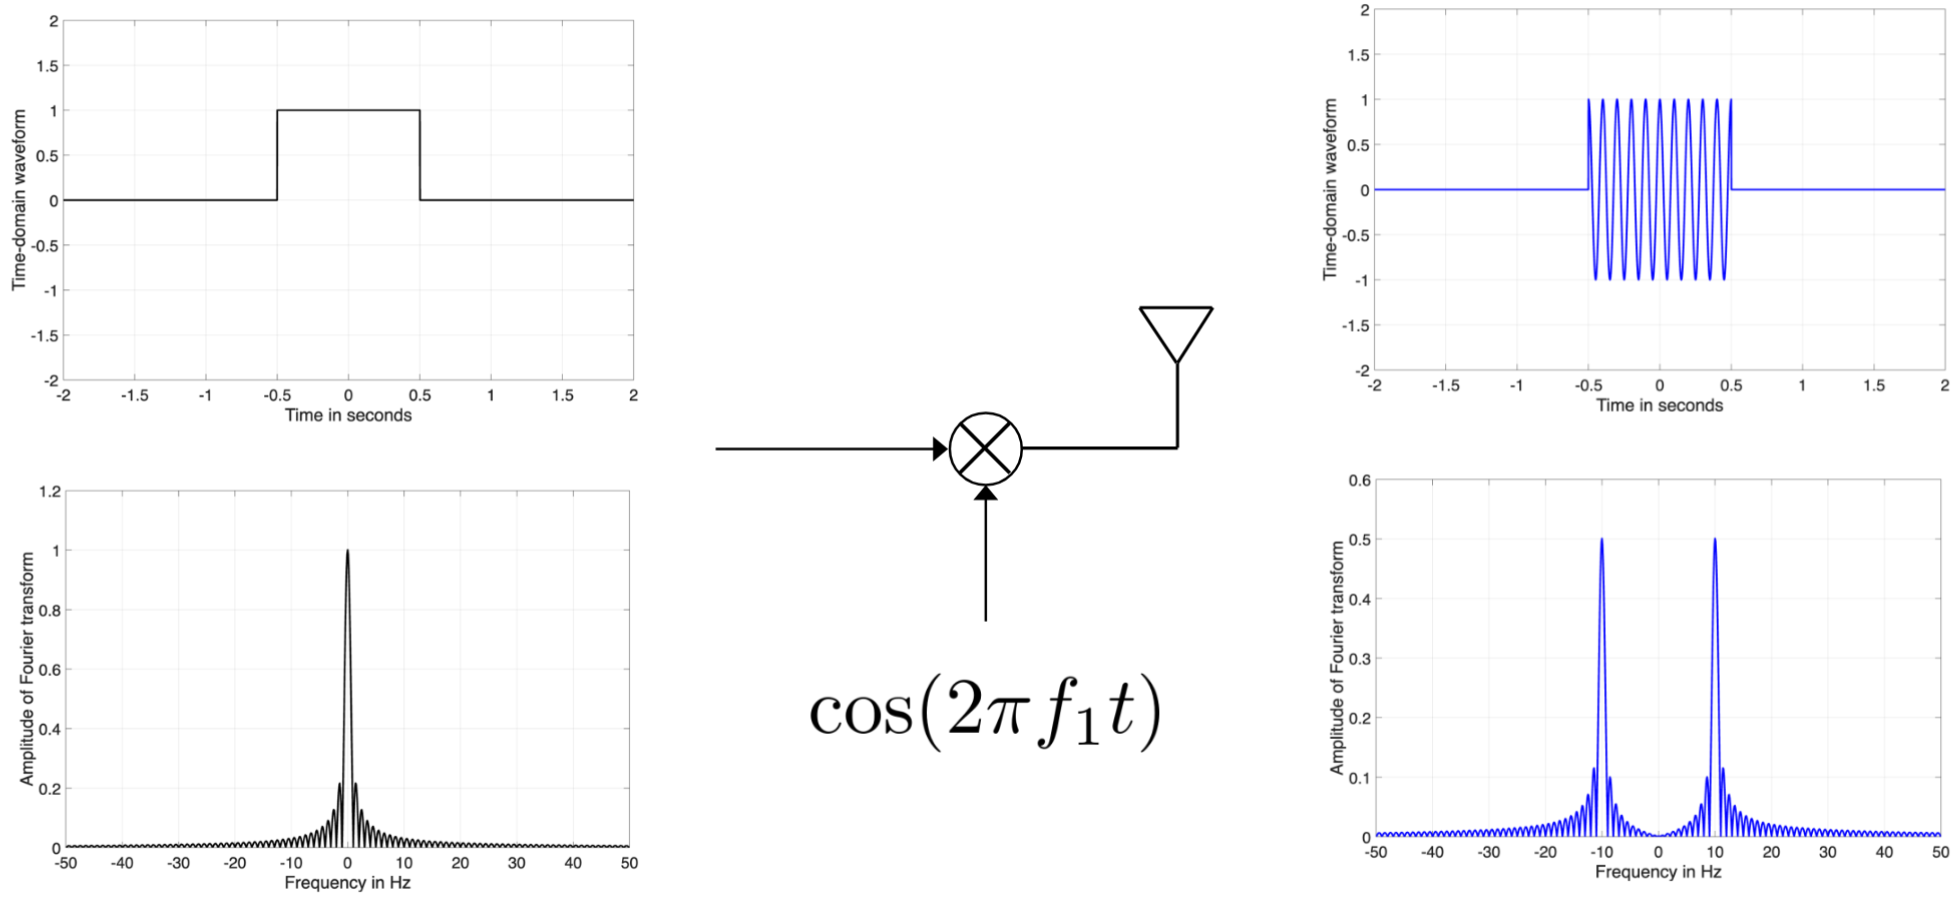
\includegraphics[scale=0.26]{../figures/modulator.png}
\end{center}
Avevamo anticipato questo dispositivo negli elementi di un sistema di comunicazione in 1.2. Questo non fa altro che moltiplicare un segnale per una oscillazione cosinusoidale ad una data frequenza $f_0$, in modo da portarne lo spettro in una regione prestabilita. In simboli:
$$
s(t) \rightarrow s(t) \cos(2 \pi f_0 t)
$$

Quindi si sfutta direttamente il teorema della modulazione per portare il segnale da un centro di frequenza attorno a zero, ad uno attorno ad $f_0$. Questo sarà quindi utile ai fini della spartizione dello spettro del mezzo di trasmissione fra più sorgenti (si pensi alla radio che trasmette su più canali). Ricordiamo inoltre che (come visto sempre in 7.6), perché la modulazione abbia l'effetto desiderato, dobbiamo scegliere frequenze di modulazione $f_0$ molto più grandi di quelle del segnale originale $f$, in modo che $f + f_0$ ci porti a destra nello spettro di frequenze (nella regione di frequenze che allochiamo al segnale) e $f - f_0$ finisca nella regione $f < 0$ (e non crei due "lobi" attorno alla $f$ originale);

	\item Corrispondente al modulatore sarà il \textbf{demodulatore}:
\begin{center}
	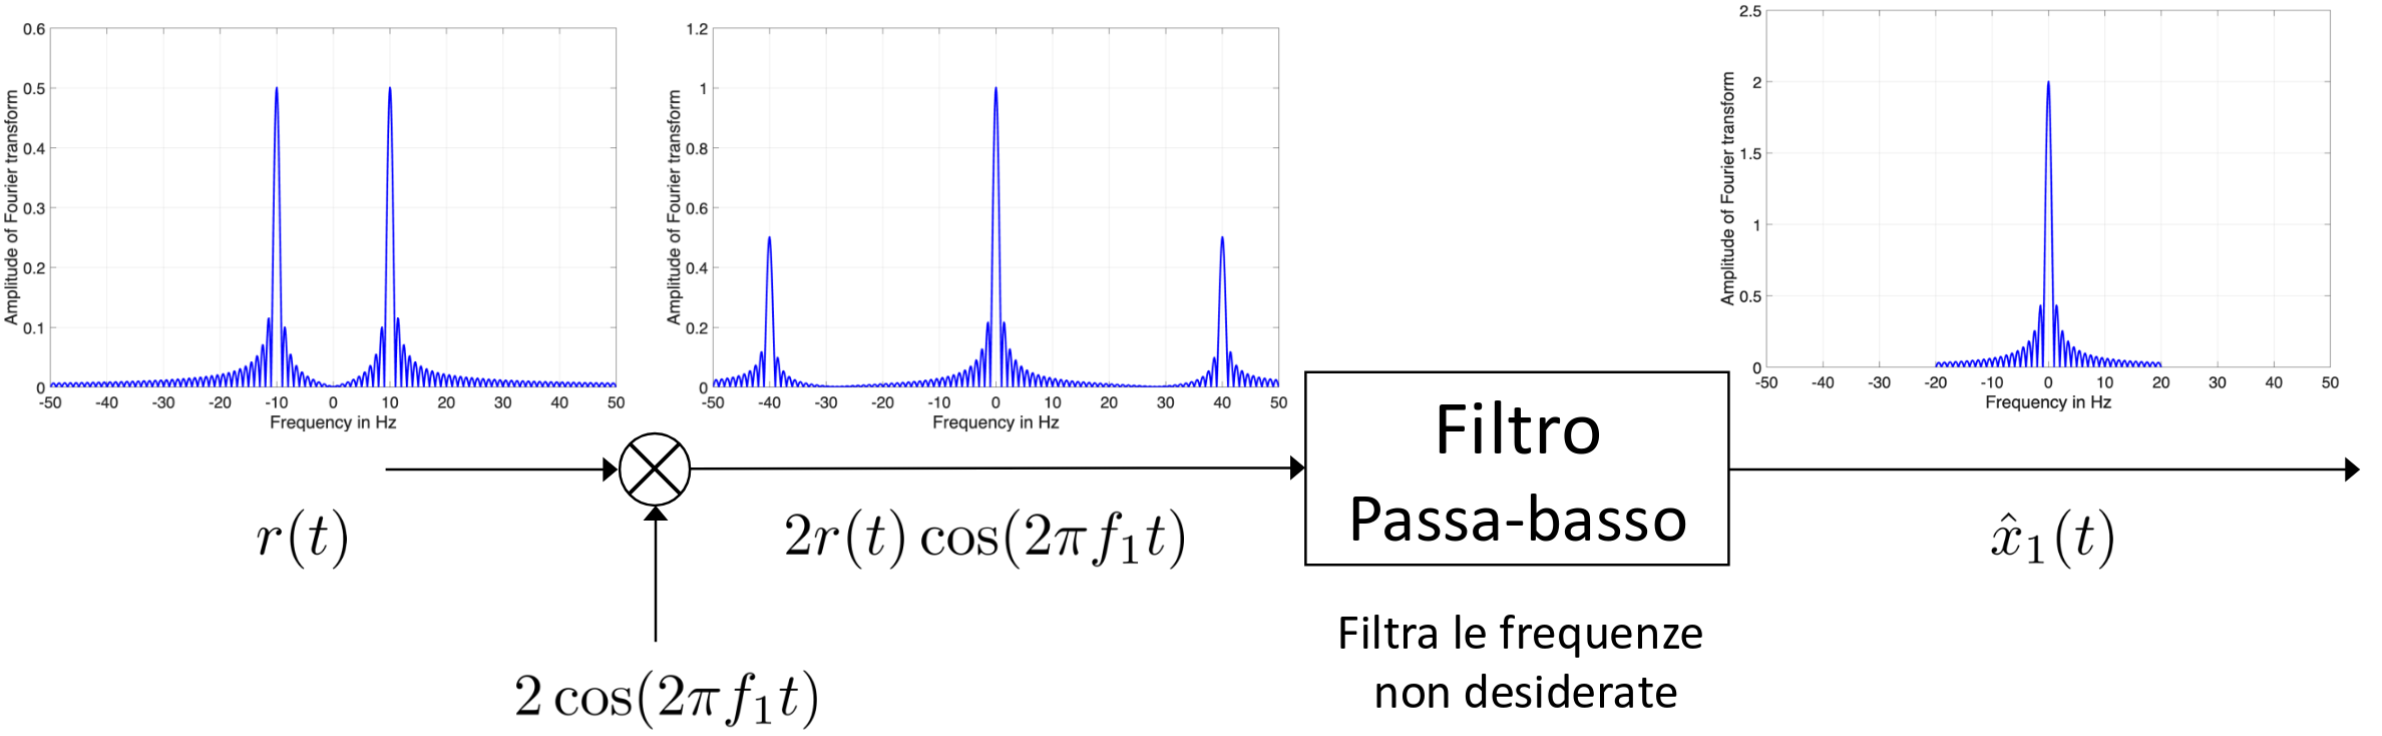
\includegraphics[scale=0.2]{../figures/demodulator.png}
\end{center}
Questo sarà un secondo dispositivo che si occupa di riportare il segnale modulato al segnale originale. Questo si può fare con una successiva moltiplicazione per $2 \cos(2 \pi f_0 t)$. Si ha infatti che il segnale $r(t)$ ricevuto dall'antenna del demodulatore è una qualche approssimazione del segnale trasmesso dal modulatore:
$$
r(t) = s(t) \cos(2 \pi f_0 t)
$$
e moltiplicando si ottiene il seguente risultato.
$$
\implies
s(t) \cdot 2 \cos(2 \pi f_0 t) = 2 s(t) \cos^2 (2 \pi f_0 t) = s(t) + s(t) \cos(4 \pi f_0 t)
$$
dalle proprietà del coseno.

Questo significa che riusciamo ad ottenere il segnale originale, più una componente ad alta frequenza ($cos(4 \pi f_0 t$). Questa verrà rimossa da un successivo stage di filtraggio passa basso, che rimuoverà la componente.

Saremmo quindi riusciti ad ottenere nuovamente il segnale demodulato (o una sua approssimazione), dopo averlo trasmesso, modulato, ad un range di frequenze specifico e selezionato dalla frequenza di modulazione $f_0$.
\end{itemize}

\subsubsection{Somma di più segnali}
Vediamo nello specifico questo processo studiando cosa succede nel caso di più segnali modulati trasmessi sullo stesso mezzo di comunicazione. Siano questi $s_1$, $s_2$ e $s_3$ funzione del tempo trasmessi da altrettante antenne collegate a modulatori. Ad ogni modulatore verrà chiaramente assegnata la sua frequenza di modulazione $f_i$. Avremo quindi che il segnale complessivo che viaggia sul mezzo condiviso sarà:
$$
\{s_1(t), s_2(t), s_3(t) \} \rightarrow s_1(t) \cos(2 \pi f_1 t) +  s_2(t) \cos(2 \pi f_2 t) +  s_3(t) \cos(2 \pi f_3 t)
$$

Quello che vedrà un demodulatore sullo stesso mezzo sarà quindi la somma dei segnali trasmessi. Potremmo chiederci allora come facciamo ad isolare un dato segnale dalla combinazione lineare di tutti i segnali che abbiamo messo in trasmissione nell'etere. La soluzione sarà dato dallo stage di filtraggio passa basso, previsto a termine del processo di demodulazione, e pensato per rimuoverà la componente ad alta frequenza che ottenevamo in:
$$
s_i(t) + s_u(t) \cos(4 \pi f_i t)
$$

L'idea è che le frequenze $4 \pi f_i$ andranno a finire distanti l'una dall'altra, per cui in fase di filtraggio dell'$i$-esimo segnale potremo rimuvoere completamente l'effetto degli altri segnali modulati, e quindi ottenere l'isolamento che ci prefissavamo di avere.

\par\smallskip

\newpage

\noindent
\textbf{\textsf{Radio}}

\noindent
Come abbiamo visto in 7.6, il teorema di modulazione ed in genere le tecniche di modulazione e demodulazione sono fondamentali al campo della trasmissione radio. Infatti, il fatto che si possano modulare segnali a diverse frequenze, assieme al teorema 7.1 (di \textit{linearità}), significa che possiamo piazzare più segnali temporali a frequenze diverse dello spettro (in questo caso dello spettro radio).

\begin{center}
	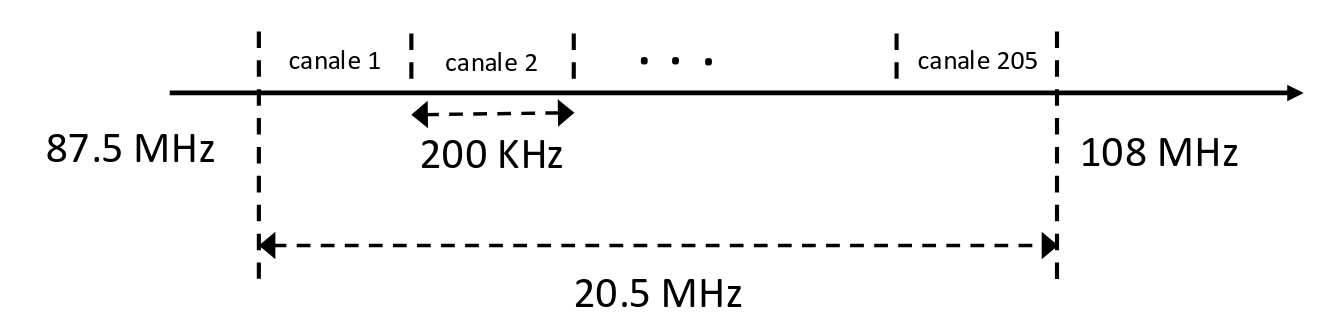
\includegraphics[scale=0.25]{../figures/spec_spec.png}
\end{center}

In particolare, nel \textit{broadcasting FM} (lo standard moderno della radio analogica) si ha una banda di frequenze che va dagli $87.5 \, \mathrm{MHz}$ ai $108 \, \mathrm{MHz}$, suddivisa in circa 205 canali che possono essere allocati alle stazioni.

\par\smallskip

\noindent
\textbf{\textsf{Reti cellulari}}


\noindent
Un utilizzo simile della modulazione viene fatto nell'accesso multiplo in divisione di frequenza (\textbf{FDMA}, \textit{Frequency Modulation Multiple Access}), usato dalle reti mobili come ad esempio il 4G LTE.

\begin{center}
	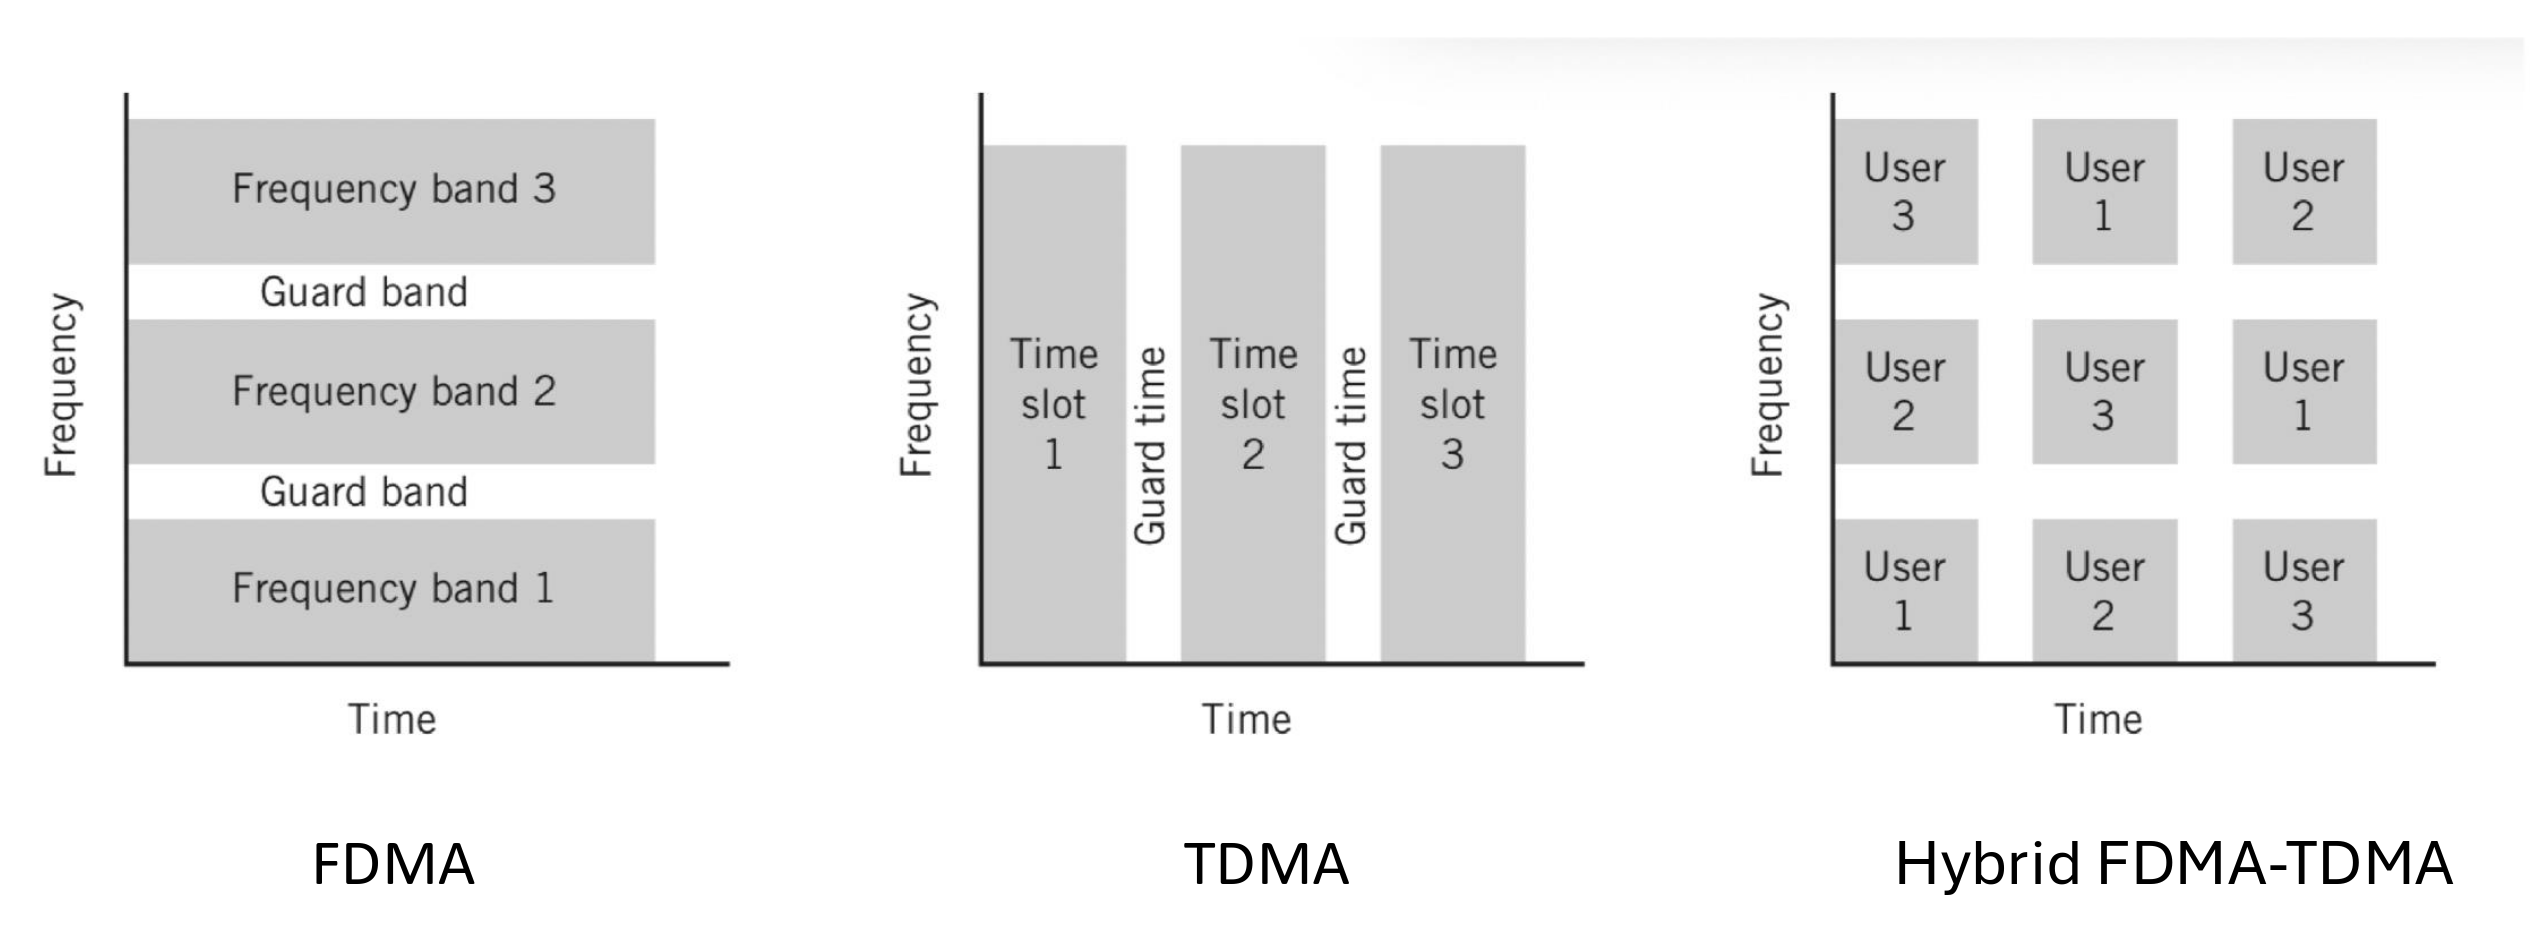
\includegraphics[scale=0.15]{../figures/4g_part.png}
\end{center}

Anche in questo caso, si divide lo spettro del mezzo in più bande di frequenza, allocata ognuna ad un diverso trasmettitore. In particolare, avevamo visto che il 4GLTE sfrutta un apporccio \textit{ibrido} FDMA-TDMA, dove si divide il mezzo sia in slot temporali che bande di frequenza, ottenendo quindi una sorta di \textit{matrice} di slot disponibili per la trasmissione. 

\subsection{Eco radar}
Nei sistemi \textbf{radar}, si invia un segnale che si propaga nello spazio finché non si incontra un ostacolo. La successiva riflessione dall'ostacolo riporta il segnale originale al ricevitore, dopo un certo tempo $\tau$.

\newpage

Poniamo di avere un segnale $x(t)$ trasmesso, equivalente alla funzione $\mathrm{rect}(\frac{t}{T})$, e di tracciare il suo eco radar $y(t)$ dopo il tempo $\tau$: 
\begin{center}
	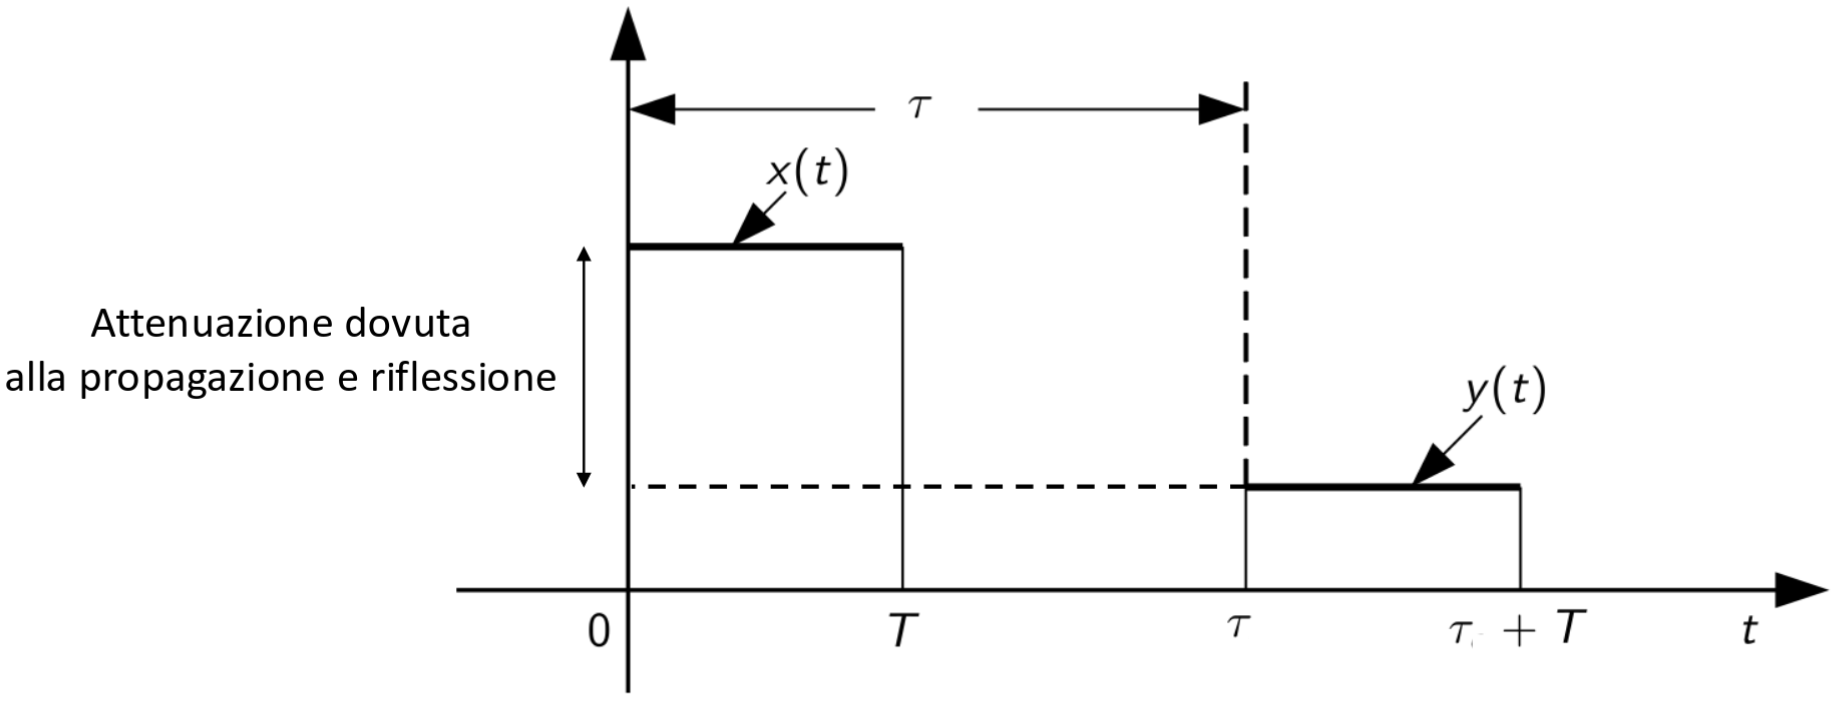
\includegraphics[scale=0.28]{../figures/radar.png}
\end{center}

Sul grafico notiamo come l'intensità del segnale $y(t)$ viene ridotta per effetto della \textit{attenuazione} di propagazione e riflessione.
In 4.1 avevamo discusso la formula di Friis, e avevamo definito il rapporto di potenza fra trasmettitore e ricevitore $\beta$:
$$
\beta = \frac{P_r}{P_t} = \frac{\lambda^2}{(4 \pi d^2)}
$$
dove la distanza $d$ non sarà altro che la distanza dell'ostacolo stesso (in questo caso il trasmettitore e il ricevitore sono nella stessa posizione).
Visto che 

Il sistema funziona quando i due segnali ($x(t)$ e $y(t)$) non si sovrappongono, ossia il segnale trasmesso $x(t)$ non si sovrappone con il segnale che si riceve $y(t)$. La condizione imposta sarà quindi:
$$
T << \tau
$$
Per calcolare $\tau$ dovremmo conoscere la velocità del segnale (poniamo $c$), e quindi dovremmo prendere come distanza $2d$ (in quanto il segnale deve \textit{arrivare} e \textit{tornare} al dispositivo). In simboli:
$$
\tau = \frac{2 d}{c}
$$

Abbiamo quindi la possibilità di trovare l'espressione esplicita di $y(t)$ in funzione di $x(t)$ e delle caratteristiche del mezzo e dell'ostacolo che incontriamo:
$$
y(t) = \sqrt{\beta} x(t - \tau)
$$
dove l'$(x - \tau)$ indica effettivamente lo scostamento temporale dato dalla distanza $2d$ complessiva che il segnale deve percorrere. Prendiamo la radice quadrata dell'attenuazione $\beta$ in quanto i segnali $x(t)$ e $y(t)$ si trovano nel dominio di potenza, e non ampiezza, per cui dobbiamo passare alle radici.

\par\smallskip

\noindent
\textbf{\textsf{Modulazione nei sistemi radar}}

\noindent
Il teorema di modulazione, di cui abbiamo visto i vantaggi nei sistemi di comunicazione per il partizionamento dello spettro dei mezzi di trasmissione, ha una sua utilità anche nei sistemi radar. Abbiamo infatti che la riflessione è migliore per segnali ad alta frequenza (questo dal $\lambda$ a numeratore del fattore di attenuazione $\beta$, maggiore frequenza significa minore attenuazione). In simboli questo si ha da:
$$
\lambda = \frac{c}{f_0}
$$

Il problema è che è molto difficile ottenere segnali che superino una certa soglia di frequenza. Di base, infatti, vorremo usare segnali $\mathrm{rect}$ che consistono in una singola oscillazione dallo zero al valore massimo (come la nostra $x(t)$), ed è improbabile ridurre ulteriormente la durata del segnale oltre una certa soglia.

La soluzione consiste nel modulare il segnale ad una frequenza maggiore, approfittando del fatto che questo porta tutto lo spettro del segnale ad una frequenza maggiore $f_0$.
In particolare notiamo i range:
\begin{itemize}
	\item $24.0 \, \mathrm{MHz}$ - $25.25 \, \mathrm{MHz}$ per il \textbf{SRR} (\textit{Short Range Radar});
	\item $76 \, \mathrm{MHz}$ - $81 \, \mathrm{MHz}$ per il \textbf{MRR} (\textit{Medium Range Radar}).
\end{itemize}

\subsection{Teorema del prodotto}
Ricolleghiamoci ai teoremi di 7.6 introducendo il cosiddetto \textit{teorema del prodotto}, che è un affermazione simile a quella del \textit{prodotto di convoluzione} sulla trasformata di Laplace:
\begin{theorem}{Prodotto della trasformata di Fourier}
	La trasformata del prodotto di due funzioni $x(t)$ e $y(t)$ è il prodotto di convoluzione (o \textit{integrale di convoluzione}) delle trasformate:
$$
z(t) = x(t) \cdot y(t) \implies Z(f) = \int_{v=-\infty}^{v=\infty} X(v) Y(f - v) \, dv = X(f) \circledast Y(f)
$$
\end{theorem}

La dimostrazione di questo risultato si ha dall'equazione di \textit{analisi}:
$$
Z(f) = \int_{t=-\infty}^{t=\infty} x(t) y(t) e^{-i 2 \pi f t} \, df
$$
in cui possiamo riscrivere il fattore $x(t)$ secondo l'equazione di \textit{sintesi}:
$$
Z(f) = \int_{t=-\infty}^{t=\infty} \left( \int_{v=-\infty}^{v=\infty} X(v) e^{i 2 \pi v t} \, dv \right) \, y(t) e^{-i 2 \pi f t} \, df
$$
$$
= \int_{v=-\infty}^{v=\infty} X(v) \left(\int_{t=-\infty}^{t=\infty} y(t) e^{-i 2 \pi (f - v)} \, dt \right) \, dv = \int_{v=-\infty}^{+\infty} X(v) Y(f - v) \, dv = X(f) \circledast Y(f)
$$
che notiamo è esattamente la tesi. \hfill $\square$

\par\smallskip

\noindent
\textbf{\textsf{Richiami sul prodotto di convoluzione}}

\noindent
Facciamo quindi alcuni richiami su cosa è esattamente il prodotto di convoluzione fa due funzioni $x(t)$ e $y(t)$ (queste non sono le funzioni della dimostrazione precedente, che moltiplicavamo in dominio tempo, ma altre 2 funzioni nel dominio tempo arbitrarie, di cui facciamo il prodotto di convoluzione). Lavoriamo nel dominio tempo anziché il dominio frequenziale in quanto è più comodo. 

% finire questa sezione

\begin{center}
	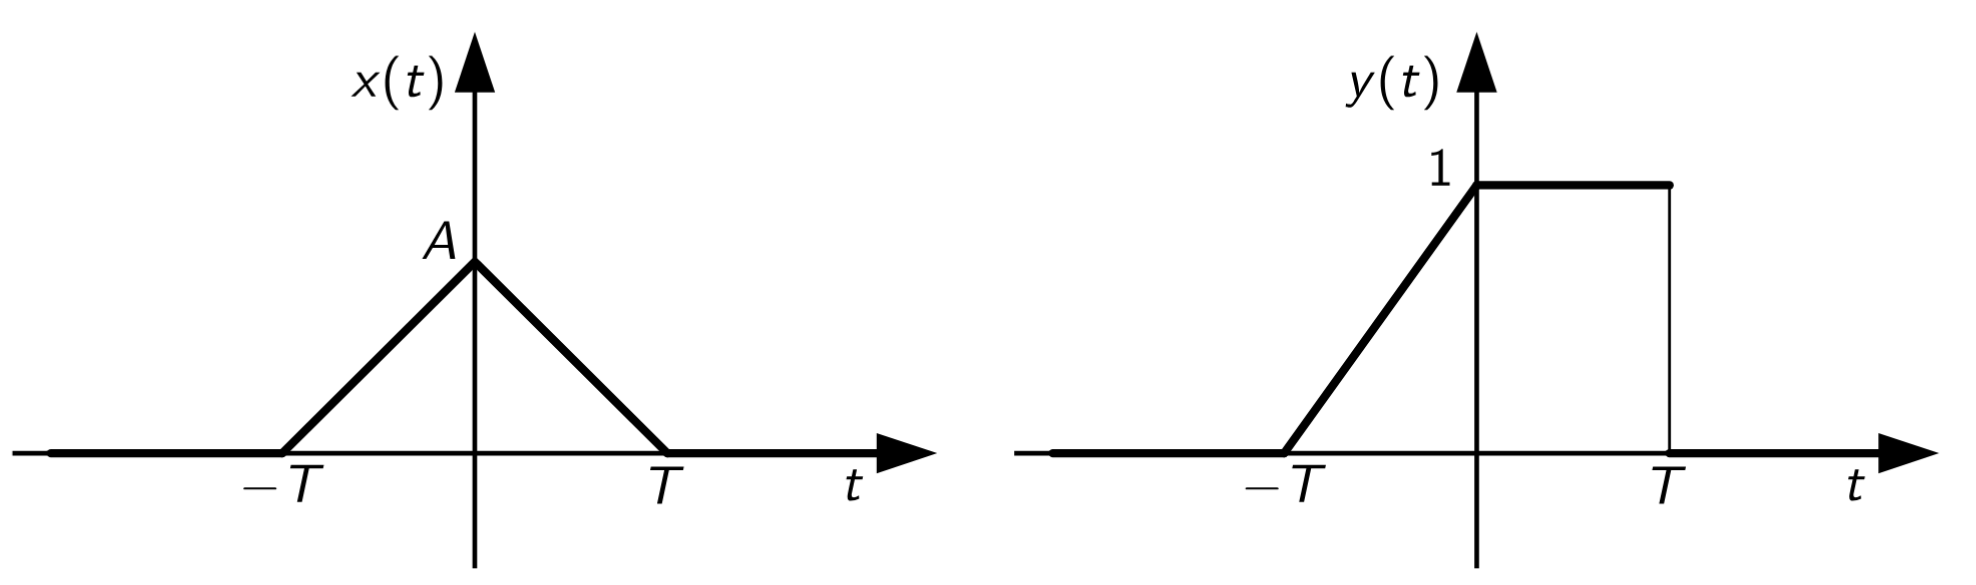
\includegraphics[scale=0.26]{../figures/conv_intro.png}
\end{center}

\begin{center}
	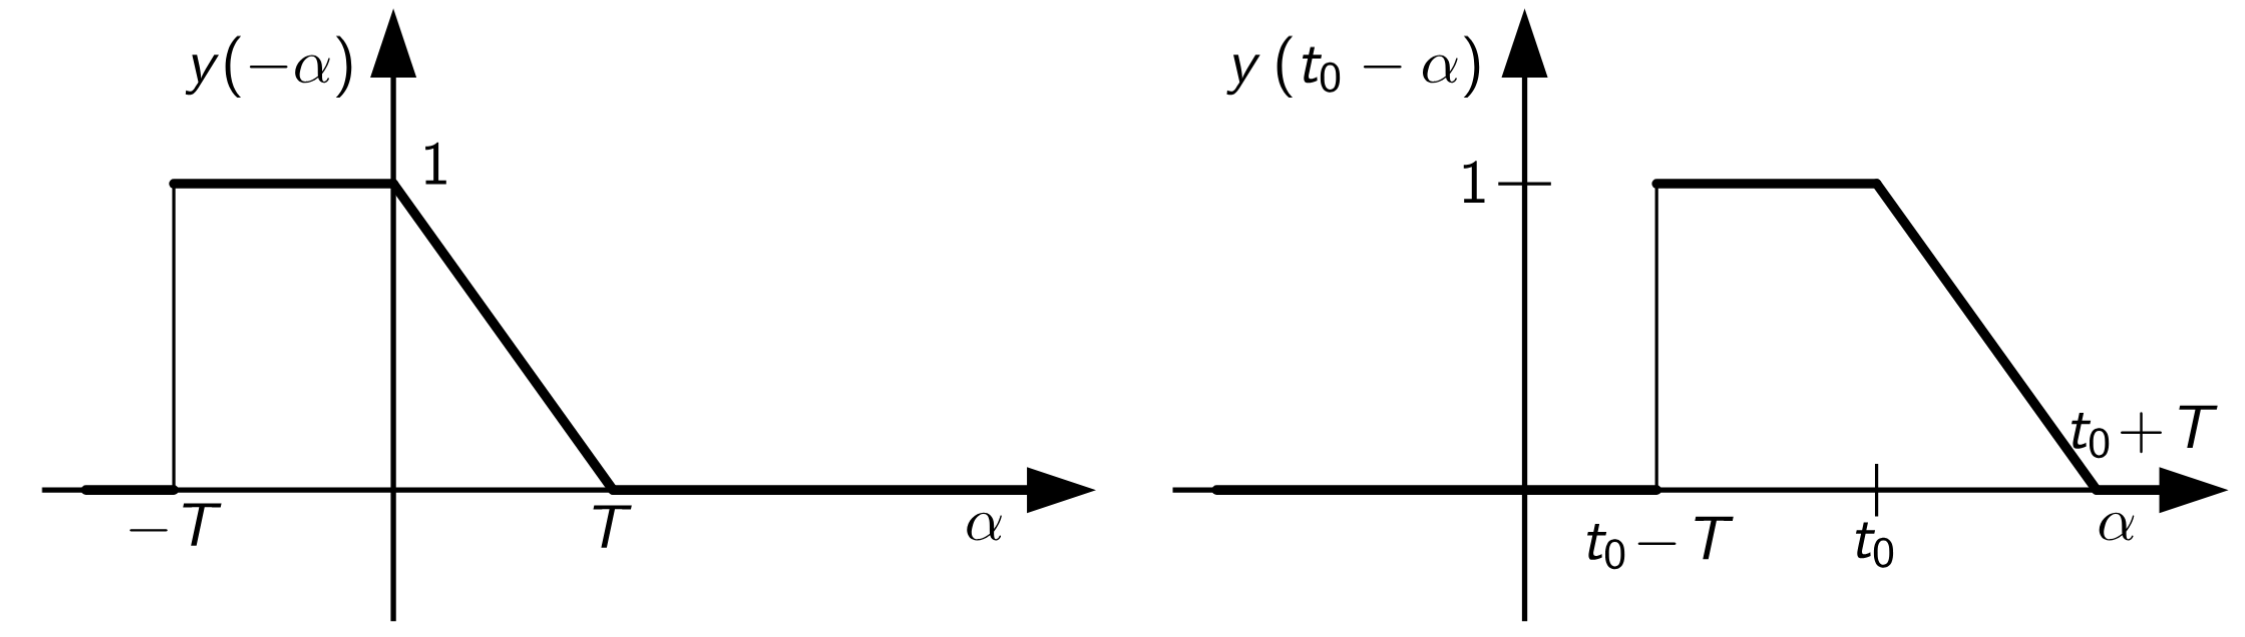
\includegraphics[scale=0.26]{../figures/conv_rev.png}
\end{center}

In generale, quindi, ricordiamo che il supporto dell’integrale di convoluzione tra due funzioni aventi estensione limitata è dato dalla somma delle estensioni delle due funzioni.

\begin{center}
	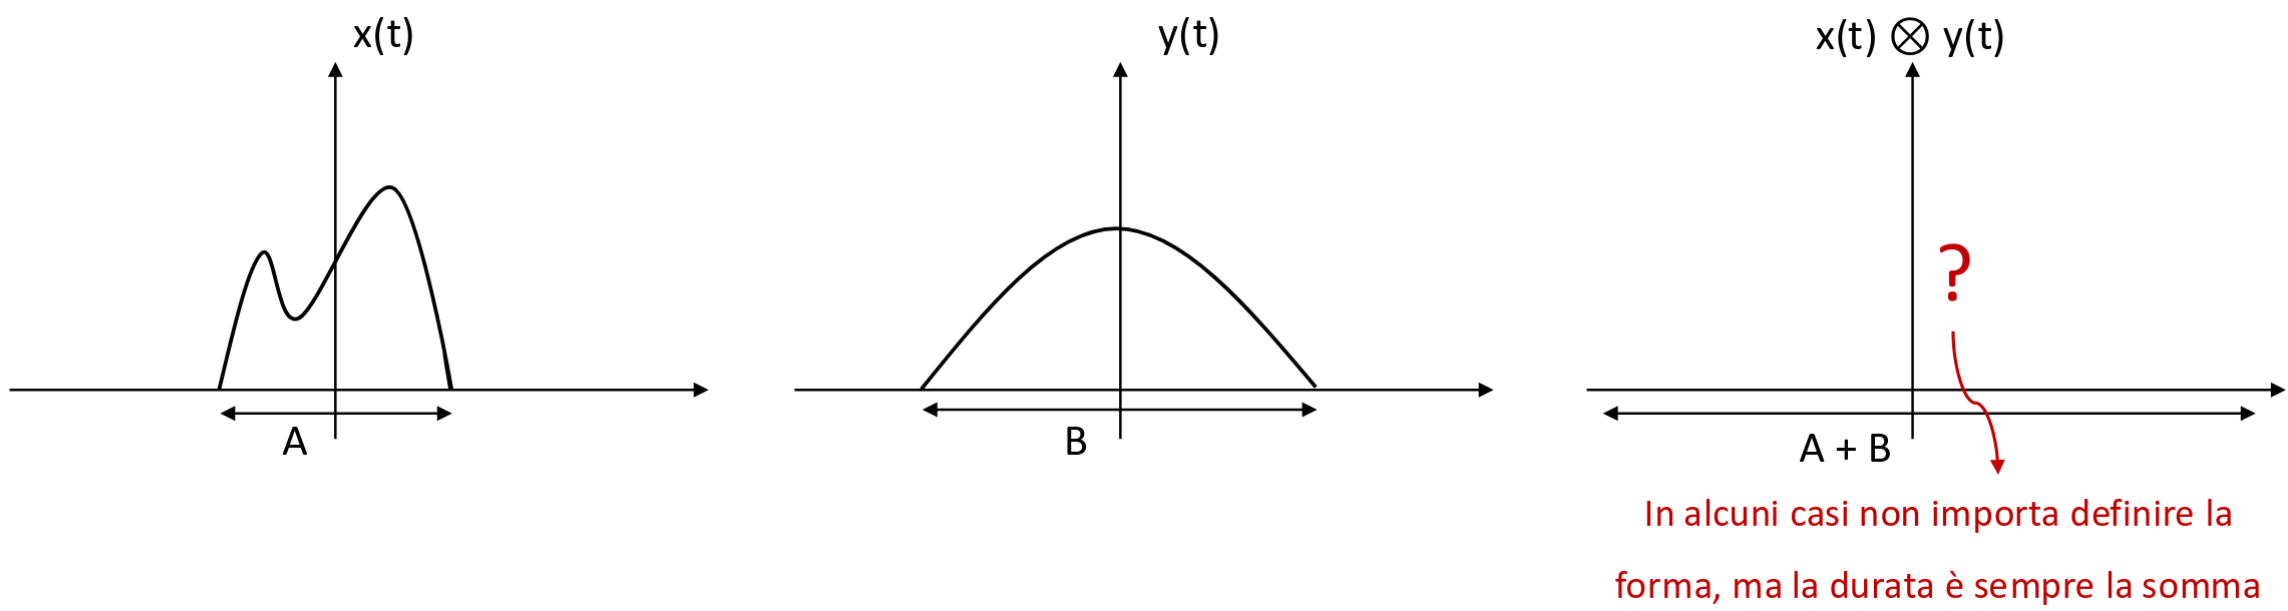
\includegraphics[scale=0.26]{../figures/conv_support.png}
\end{center}

\par\smallskip

\noindent
\textbf{\textsf{Esempi di convoluzione}}

\noindent
Vediamo quindi alcuni esempi significativi di prodotto di convoluzione fra due funzioni $x(t)$ e $y(t)$.

\begin{enumerate}
	\item % esempio 1
	\item % esempio 2
\end{enumerate}

\subsubsection{Teorema della convoluzione}
Vediamo qual'è il duale del teorema del prodotto per la trasformata di Fourier, cioè il \textit{teorema della convoluzione}:
\begin{theorem}{Convoluzione della trasformata di Fourier}
La trasformata della convoluzione di due funzioni $x(t)$ e $y(t)$ è il prodotto delle trasformate:
$$
z(t) = x(t) \circledast y(t) \implies Z(f) = \int_{\alpha=-\infty}^{\alpha=\infty} x(\alpha) y(t - \alpha) \, d\alpha = Z(f) = X(f) \cdot Y(f)
$$
\end{theorem}

Cioè alla convoluzione nel tempo corrisponde il prodotto delle trasformate. Questo è un altro risultato fondamentale per i sistemi lineari e tempo invarianti, e si dimostra direttamente dal teorema del prodotto della trasformata di Fourier in 10.1

\subsection{Definizione di banda}
Prendiamo un segnale $x(t)$ a durata finita. Ad esempio, il modo per assicurarsi di avere durata finita può essere moltiplicare per la funzione $\mathrm{rect}$ (che per definizione ha durata finita).

\begin{center}
	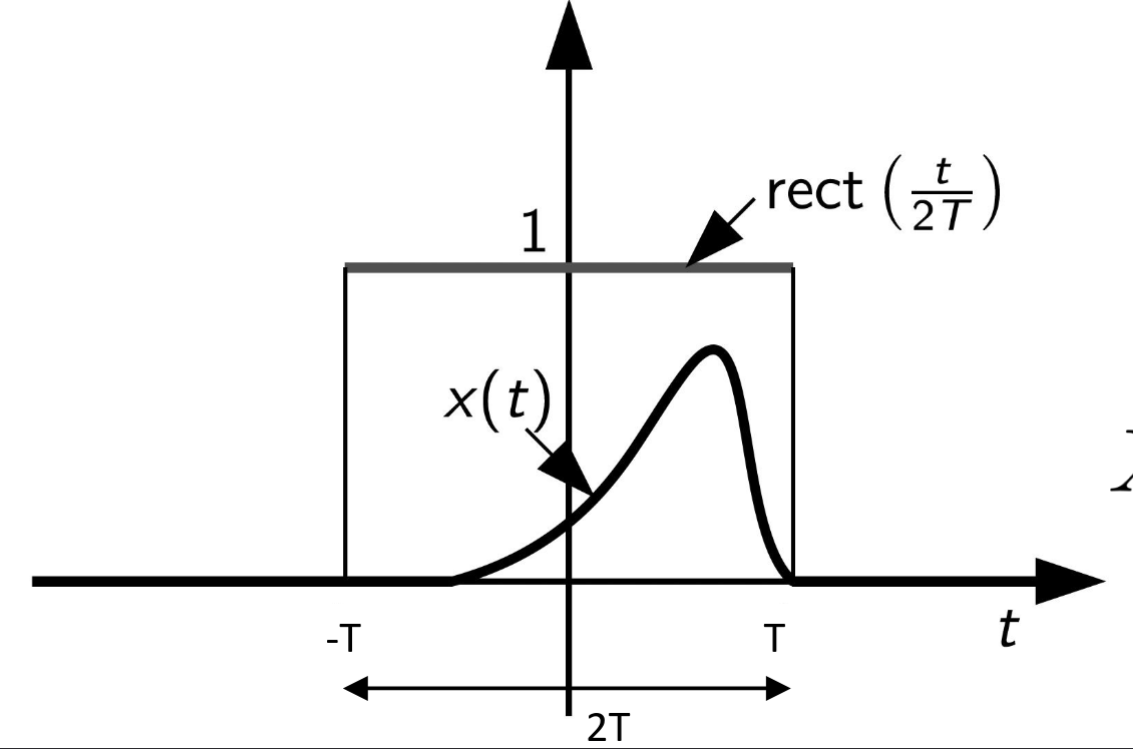
\includegraphics[scale=0.26]{../figures/finite_signal.png}
\end{center}

Il problema su cui ci interroghiamo è se questo segnale ha anche \textit{spettro} finito. Questo è automaticamente impossibile, in quanto dalle prime definizioni viste in 6.1.1 si ha che la trasformata della funzione $\mathrm{rect}$ è la funzione $\mathrm{sinc}$, che ha spettro infinito.

Prendere il segnale moltiplicato per la funzione $\mathrm{rect}$, cioè in simboli:
$$
z(t) = x(t) \mathrm{rect}\left( \frac{t}{\frac{T}{2}} \right)
$$
equivale a prendere la $y(t) = \mathrm{rect}\left( \frac{t}{\frac{T}{2}} \right)$ nel teorema del prodotto e quindi ottenere il prodotto di convoluzione:
$$
X(f) = X(f) \circledast 2 T \matrm{sinc}(2 f T)
$$
che ha per forza banda infinita da quanto detto prima: il supporto dell’integrale di convoluzione tra due funzioni aventi estensione limitata è dato dalla somma delle estensioni delle due funzioni.

Nel mondo reale, tutti i segnali che considereremo saranno a durata finita. Abbiamo quindi bisogno di una definizione che ci permetta di prendere l'\textit{estensione} degli spettri dei segnali reali, senza considerarli sempre come infiniti.

\subsubsection{Banda a -3 dB}
Definiamo quindi la \textbf{banda a -3 dB} come il punto del grafico della potenza in funzione della frequenza $f$ che tocca i $-3 \, \mathrm{dB}$ rispetto agli $0 \, \mathrm{dB}$. Scegliamo esattamente $-3 \, \mathrm{dB}$ in quanto ricordiamo che, riguardo alle potenze:
$$
\frac{| X(B_{-3 \, \mathrm{dB}}) |^2}{| X(f_0) |^2} = \frac{1}{2}
$$
$$
\implies 10 \log_{10} \left( \frac{| X(B_{-3 \, \mathrm{dB}}) |^2}{| X(f_0) |^2} \right) \approx -3 \, \mathrm{dB}
$$
cioè i $-3 \, \mathrm{dB}$ equivalgono a raggiungere metà della potenza massima. Notiamo che si è preso $|X(f_0)|^2$ come punto agli $0 \, \mathrm{dB}$, dove $f_0$ sarà la frequenza alla quale vorremo campionare la potenza massima. Solitamente si ha $f_0 = 0$.

\begin{center}
	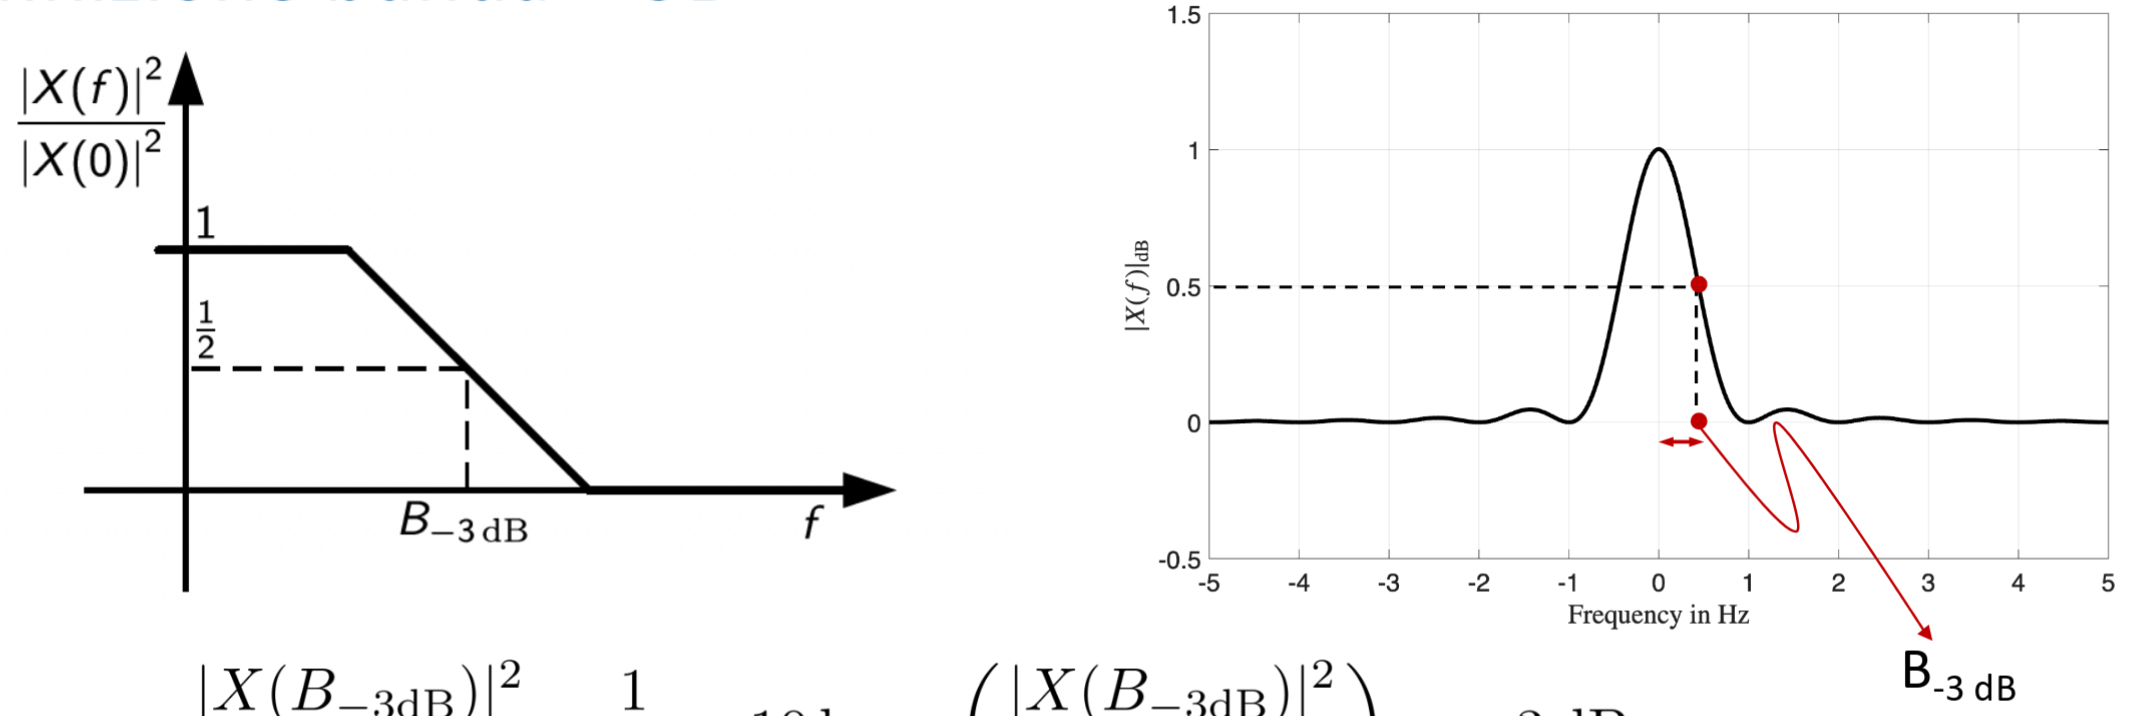
\includegraphics[scale=0.26]{../figures/band3db.png}
\end{center}

Da un punto di vista meno teorico, la banda a $-3 \, \mathrm{dB}$ rappresenta un’indicazione “pratica” della banda di un segnale: frequenze inferiori alla banda sono ritenute “importanti”, mentre quelle superiori sono ritenute “trascurabili”. Esistono anche altri tipi di banda, come ad esempio la banda a $-1 \, \mathrm{dB}$, la banda al 99\% dell'energia, ecc...

\subsubsection{Banda a -3 dB per segnali modulati}
Per un segnale modulato abbiamo che l'intera banda, come dal teorema di modulazione, viene spostata della freuenza modulante $f_0$.
Ciò che accadrà per la nostra definizione di banda a $-3 \, \mathrm{dB}$ sarà che in :
$$
\frac{| X(B_{-3 \, \mathrm{dB}}) |^2}{| X(f_0) |^2} = \frac{1}{2}
$$
prenderemo $f_0$ alla frequenza modulante.

Un altra caratteristica è che per i segnali modulati, quindi, possiamo identificare due limiti di banda a $-3 \, \mathrm{db}$: quello sopra $f_0$ e quello sotto.
Come conseguenza si ha un’\textit{ampiezza di banda} a $-3 \, \mathrm{dB}$ come differenza tra i due limiti.

\subsubsection{Banda al 99\% dell'energia}
Vediamo un'altra definizione di banda, che avevamo anticipato, e che deriva da un \textit{criterio energetico}. Questa sarà la \textbf{banda al 99\% dell'energia}:
$$
\int_{-B_{99}}^{B_{99}} |X(f)|^2 \, df = 0.99 E_x = 0.99 \int |X(f)|^2 \, df
$$

Dal teorema di Parseval (teorema 6.1) avevamo che l'energia sul dominio temporale è uguale a quella sul dominio frequenziale. Quindi, possiamo dare una definizione di banda anche prendendo gli estremi che racchiudono il 99\% dell'energia di un segnale. Saranno questi gli estremi della banda al 99\% come volevamo definire.

\end{document}
